\documentclass[11pt]{article}
\usepackage[margin=1in]{geometry}
\usepackage{graphicx}
\usepackage{microtype}
\usepackage{verbatim}
\usepackage{amsmath}
\usepackage{nicefrac}
\usepackage[colorlinks=false, hidelinks]{hyperref}
\usepackage{caption}
\usepackage{subcaption}
\usepackage{listings}
\usepackage{harmony}
\usepackage{wasysym}

\begin{document}

\title{Tricycle Lights\\Embedded System Design, Lab 6}
\date{October 29, 2015}
\author{Ben Lorenzetti}
\maketitle

\tableofcontents

\clearpage

\section{Objectives and Problem Description}
\label{problem-specs}

\subsection{Tricycle Lights}

Blink two LEDs, representing left and right turn signals,
depending on the position of a rotary potentiometer,
which represents a steering wheel. The following conditions should be met.

\begin{enumerate}
\item
Use the potentiometer and LEDs on the 44--Pin Demo Board.
\item
Use the LED connected to RD7 for the left turn signal, and RD0 for right.
\item
When wheel is in neutral position (wiper in middle of pot.),
both turn indicator lights should be off.
\item
When turned counterclockwise or clockwise from neutral position,
the left or right LEDs should blink at a rate proportional to the
angular displacement from neutral position.
\end{enumerate}

\section{Procedure}

\subsection{Potentiometer and LEDs on the 44--Pin Demo Board}

\begin{figure}
\centering
	\begin{subfigure}[b]{.3\textwidth}
		\centering
		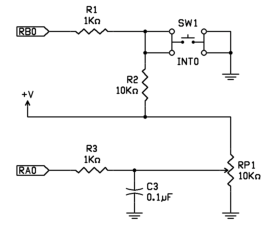
\includegraphics[width=\textwidth]{Figures/demo-board-pot-pushbutton-circuit.pdf}
		\caption[]%
		{{\small Potentiometer Input}}
	\end{subfigure}
	\quad
	\begin{subfigure}[b]{0.3\textwidth}
		\centering
		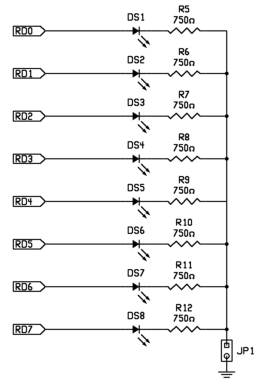
\includegraphics[width=\textwidth]{Figures/demo-board-led-circuit.pdf}
		\caption[]%
		{{Output LEDs}}
	\end{subfigure}	
	\caption{I/O Circuit Diagrams from the 44--Pin Demo Board User's Manual}
	\label{io-circuit-diagram}
\end{figure}

In this lab, we will need to measure a potentiometer input (the steering wheel)
and blink two LEDs for output. The 44--pin demo board for the PIC16F887
has all of this hardware on board. The potentiometer and LEDs are connected to
pins as shown in the circuit diagram in
\hyperref[io-circuit-diagram]{figure \ref{io-circuit-diagram}}.

According to the specifications, the LED at RD7 should be the left blinker
and the LED at RD0 should be the right blinker.

\subsection{PIC16F887 Analog to Digital Converter (ADC)}



\subsection{PIC16F887 Clock Sources}

\subsection{Implementation Flowchart}

\subsection{Delay Function}

\subsection{Linear Mapping}

\section{Expected Results}

\section{Experiment and Design Revisions}

\subsection{Command Line Assembly}

My \texttt{.asm} source files were assembled on the command line so
please do this if they don't compile nicely in the IDE.
On Ubuntu, with the default MPLAB installation location, 
from the directory containting \texttt{lfsr.asm}, the commands are:
\begin{verbatim}
$ cp /opt/microchip/mplabx/v3.10/mpasmx/p16f887.inc ./p16f887.inc
$ /opt/microchip/mplabx/v3.10/mpasmx/mpasmx -p16f887 lfsr.asm
$ more lfsr.ERR
\end{verbatim}

\section{Observations}

\begin{center}
	\includegraphics[width=0.5\textwidth]{Figures/tricycle-lights-demo.jpg}
	\captionof{figure}{Demonstration of Tricycle Turn Lights}
	\label{tricycle-lights-jpg}
\end{center}

\section{Discussion}

\clearpage

\section{Tricycle Lights Implementation Code}
\label{implementation-code}

\lstinputlisting[breaklines, basicstyle=\small]{Tricycle-Lights/tricycle-lights.asm}

\end{document}
